%%%%%%%%%%%%%%%%%%%%%%%%%%%%%%%%%%%%%%%%%%%%%%%%%%%%%%%%%%%%%%%%%
\section{Code}		%	Code
%%%%%%%%%%%%%%%%%%%%%%%%%%%%%%%%%%%%%%%%%%%%%%%%%%%%%%%%%%%%%%%%%
Der in diesem Abschnitt präsentierte Teil des in dieser Arbeit verwendeten Codes soll zur besseren Gesamtverständlichkeit dieser Arbeit beitragen.

\subsection{\Rm}
Anbei die Realisierung der zweiten und dritten Phase des Algorithmus \Rm durch die Methoden \pythoninline{def rmin_phase2} und \pythoninline{def rmin_phase3}.

\subsubsection{Phase 2}
\documentclass[border=3pt]{standalone}
\usepackage{tikz}
\usetikzlibrary{decorations.pathreplacing,patterns}
\definecolor{greengreen}{rgb}{0.0, 0.42, 0.24}
%%%%%%%%%%%%%%%%%%%%%%%%%%%%%%%%%%%%%%%%%%%%%%%%%%%%%%%%%%%%%%%%%
\begin{document}
%%%%%%%%%%%%%%%%%%%%%%%%%%%%%%%%%%%%%%%%%%%%%%%%%%%%%%%%%%%%%%%%%
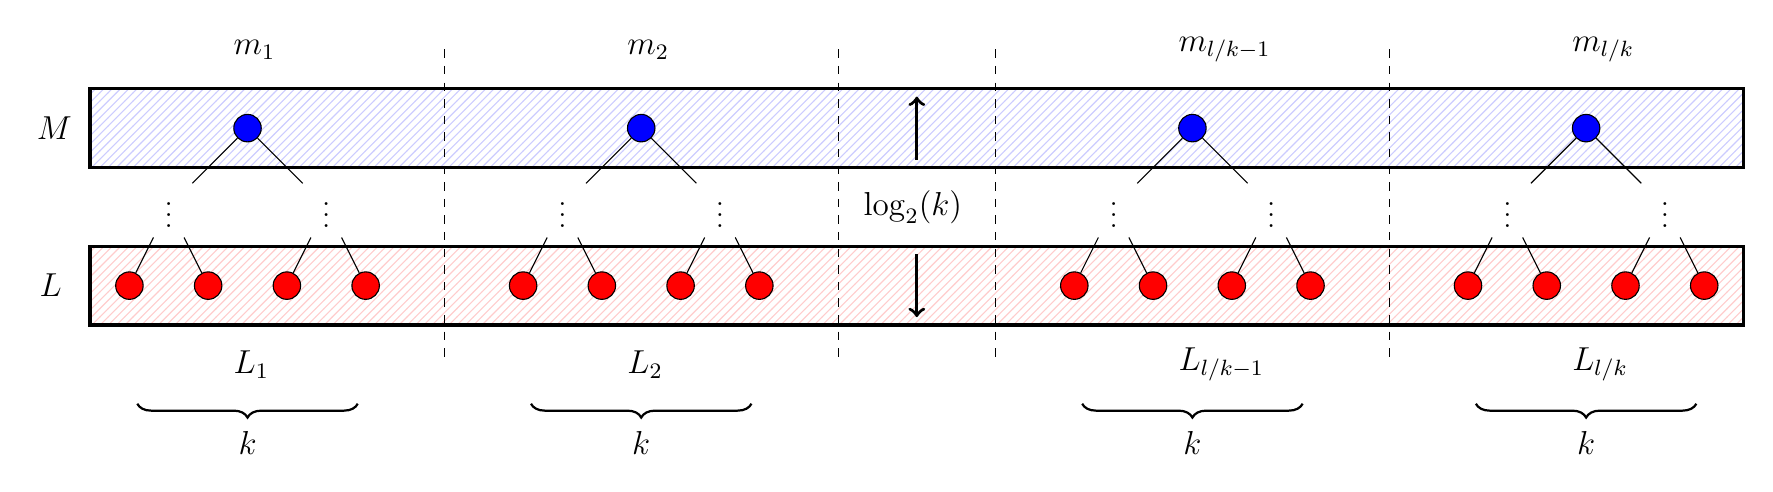
\begin{tikzpicture}[every node/.style={align=center},
red/.style={fill=red,draw,circle,inner sep=0pt},
blue/.style={fill=blue,draw,circle,inner sep=0pt},
 text width = .35cm]
%================================================================
%	Boxes
\draw[very thick, pattern=north east lines, pattern color=red!20] (-0.5,-0.5) rectangle (20.5,0.5);
\draw[very thick, pattern=north east lines, pattern color=blue!20] (-0.5,1.5) rectangle (20.5,2.5);

%================================================================
%	Nodes
\node[style=red] (r1) at (0,0) {};
\node[style=red] (r2) at (1,0) {};
\node[style=red] (r3) at (2,0) {};
\node[style=red] (r4) at (3,0) {};
\node[style=red] (r5) at (5,0) {};
\node[style=red] (r6) at (6,0) {};
\node[style=red] (r7) at (7,0) {};
\node[style=red] (r8) at (8,0) {};
\node[style=red] (r9) at (12,0) {};
\node[style=red] (r10) at (13,0) {};
\node[style=red] (r11) at (14,0) {};
\node[style=red] (r12) at (15,0) {};
\node[style=red] (r13) at (17,0) {};
\node[style=red] (r14) at (18,0) {};
\node[style=red] (r15) at (19,0) {};
\node[style=red] (r16) at (20,0) {};
%----------------------------------------------------------------
\node (d1) at (0.5,1) {$\vdots$};
\node (d2) at (2.5,1) {$\vdots$};
\node (d3) at (5.5,1) {$\vdots$};
\node (d4) at (7.5,1) {$\vdots$};
\node (d5) at (12.5,1) {$\vdots$};
\node (d6) at (14.5,1) {$\vdots$};
\node (d7) at (17.5,1) {$\vdots$};
\node (d8) at (19.5,1) {$\vdots$};
%----------------------------------------------------------------
\node[style=blue] (b1) at (1.5,2) {};
\node[style=blue] (b2) at (6.5,2) {};
\node[style=blue] (b3) at (13.5,2) {};
\node[style=blue] (b4) at (18.5,2) {};

%================================================================
%	Lines
\draw (r1) -- (d1);
\draw (r2) -- (d1);
\draw (r3) -- (d2);
\draw (r4) -- (d2);
\draw (r5) -- (d3);
\draw (r6) -- (d3);
\draw (r7) -- (d4);
\draw (r8) -- (d4);
\draw (r9) -- (d5);
\draw (r10) -- (d5);
\draw (r11) -- (d6);
\draw (r12) -- (d6);
\draw (r13) -- (d7);
\draw (r14) -- (d7);
\draw (r15) -- (d8);
\draw (r16) -- (d8);
%----------------------------------------------------------------
\draw (d1) -- (b1);
\draw (d2) -- (b1);
\draw (d3) -- (b2);
\draw (d4) -- (b2);
\draw (d5) -- (b3);
\draw (d6) -- (b3);
\draw (d7) -- (b4);
\draw (d8) -- (b4);
%----------------------------------------------------------------
\draw[dashed] (4,3) -- (4,-1);
\draw[dashed] (9,3) -- (9,-1);
\draw[dashed] (11,3) -- (11,-1);
\draw[dashed] (16,3) -- (16,-1);

%================================================================
%	Decoration
\draw[thick, decorate,decoration={brace,amplitude=5pt,mirror}] (0.1,-1.5) -- (2.9,-1.5);
\draw[thick, decorate,decoration={brace,amplitude=5pt,mirror}] (5.1,-1.5) -- (7.9,-1.5);
\draw[thick, decorate,decoration={brace,amplitude=5pt,mirror}] (12.1,-1.5) -- (14.9,-1.5);
\draw[thick, decorate,decoration={brace,amplitude=5pt,mirror}] (17.1,-1.5) -- (19.9,-1.5);

\draw[->, very thick] (10, 1.6) -- (10, 2.4);
\draw[->, very thick] (10, 0.4) -- (10, -0.4);
\node at (9.5,1) {\large $\log_2(k)$};
%----------------------------------------------------------------
\node at (-1,2) {\large $M$};
\node at (-1,0) {\large $L$};
%----------------------------------------------------------------
\node at (1.5,3) {\large $m_1$};
\node at (6.5,3) {\large $m_2$};
\node at (13.5,3) {\large $m_{l/k-1}$};
\node at (18.5,3) {\large $m_{l/k}$};
%----------------------------------------------------------------
\node at (1.5,-1) {\large $L_1$};
\node at (6.5,-1) {\large $L_2$};
\node at (13.5,-1) {\large $L_{l/k-1}$};
\node at (18.5,-1) {\large $L_{l/k}$};
%----------------------------------------------------------------
\node at (1.5,-2) {\large $k$};
\node at (6.5,-2) {\large $k$};
\node at (13.5,-2) {\large $k$};
\node at (18.5,-2) {\large $k$};
%================================================================
\end{tikzpicture}
%%%%%%%%%%%%%%%%%%%%%%%%%%%%%%%%%%%%%%%%%%%%%%%%%%%%%%%%%%%%%%%%%
\end{document}
%%%%%%%%%%%%%%%%%%%%%%%%%%%%%%%%%%%%%%%%%%%%%%%%%%%%%%%%%%%%%%%%%
\subsubsection{Phase 3}
\begin{python}
#   Import
import random

# ==================================================
#   RMinimum: Phase 3
def rmin_phase3(W, k, M, cnt):

    # Generate subsets
    random.shuffle(W)
    W_i = [W[i * k:(i + 1) * k] 
    		for i in range((len(W) + k - 1) // k)]
    W_i_filt = [0 for _ in range(len(W_i))]

    # Filter subsets
    for i in range(len(W_i_filt)):
        W_i_filt[i] = [elem for elem in W_i[i] if elem < M[i]]
        cnt[M[i]] += len(W_i[i])
        for elem in W_i[i]:
            cnt[elem] += 1

    # Merge subsets
    Wnew = [w for sublist in W_i_filt for w in sublist]

    return Wnew, cnt

\end{python}

\newpage
%%%%%%%%%%%%%%%%%%%%%%%%%%%%%%%%%%%%%%%%%%%%%%%%%%%%%%%%%%%%%%%%%
\subsection{\RM}
Anbei die Realisierung der zweiten Phase des Algorithmus \RM durch die Methoden \pythoninline{def rmed_phase3}.
\subsubsection{Phase 2}
\begin{python}
#   Import
import random

# ==================================================
#   RMedian: Phase 2
def rmed_phase2(S, XS, L, C, R, cnt):

    mark = [False for _ in range(len(XS) + len(S))]
    random.shuffle(XS)
    b = len(L)
    
    #	Loop
    for x_i in XS:
        med = 0	#	Check if remaining or discarded
        for j in reversed(range(0, b - 1)):

            current = 2 ** 50	# Arbitrary value
            random.shuffle(L[j])
            for l in L[j]:
                if cnt[l] < current:
                    x_A = l

            if mark[x_A] == True:
                c = 1

            else:
                c = 2

            cnt[x_i] += 1
            cnt[x_A] += 1

            if x_i < x_A:
                if j + c < b:
                    mark[x_i] = True
                    L[j + c].append(x_i)
                    med = -1
                else:
                    med = -2
                break

            current2 = 2 ** 50	# Arbitrary value
            random.shuffle(R[j])
            for r in R[j]:
                if cnt[r] < current2:
                    x_B = r

            if mark[x_B] == True:
                c = 1
            else:
                c = 2

            cnt[x_i] += 1
            cnt[x_B] += 1

            if x_i > x_B:
                if j + c < b:
                    mark[x_i] = True
                    R[j + c].append(x_i)
                    med = 1
                else:
                    med = 2
                break
        
        #	Sort remaining elements in C 
        # 	and discarded in the outer buckets.
        if med == 0:
            C.append(x_i)
        elif med == -2:
            L[len(L) - 1].append(x_i)
        elif med == 2:
            R[len(R) - 1].append(x_i)
    
    return S, XS, L, C, R, cnt
\end{python}

\newpage
%%%%%%%%%%%%%%%%%%%%%%%%%%%%%%%%%%%%%%%%%%%%%%%%%%%%%%%%%%%%%%%%%
\subsection{Werkzeug}
Neben den Algorithmen wurden weitere Werkzeuge zur Datenverarbeitung implementiert.\\[.05cm]
Anbei beispielhaft das \textit{Bash}-Skript, welches genutzt wurde, um mit dem \textit{Goethe-HLR} Cluster zu kommunizieren, sowie eine \textit{Gnuplot}-Datei~\cite{gnu} zur Berechnung eines Fits mithilfe des \textit{Marquardt-Levenberg} Algorithmus~\cite{gnu2}. 
\subsubsection{Server}
\textit{Bash}-Skript zur Ausführung der Datei \textit{python\_py1.py} auf dem \textit{Goethe-HLR} Cluster.
\begin{lstlisting}[style=bsh]
#!/bin/bash
#SBATCH --partition=general1
#SBATCH --nodes=1
#SBATCH --ntasks=40
#SBATCH --cpus-per-task=1
#SBATCH --mem=100000
#SBATCH --time=10:00:00
#SBATCH --mail-type=FAIL

export OMP_NUM_THREADS=1
export PYTHONHOME=/home/memhierarchy/lorenz/venv
export PYTHONPATH=/home/memhierarchy/lorenz/venv/python

# Run 10 times
/home/memhierarchy/lorenz/venv/bin/python py1.py >& 01.out &
...
/home/memhierarchy/lorenz/venv/bin/python py1.py >& 01.out &

# Wait for all child processes to terminate.
wait
\end{lstlisting}
\subsubsection{Fit}
\textit{Gnuplot}-Skript zur Berechnung eines Fits bezüglich der Daten aus der Datei \textit{filename.csv} und der Funktion $f(x)=a\cdot \log_2(x)/\log_2\log_2(x) + b$ mit Startwerten $a=6.5$ sowie $b=-8.5$.
\input{snippets/code/gnu}
